% !TEX root = SegwayDoku.tex
\newpage
\renewcommand{\autoren}{Valentyn Chepil}
\section{Die Gehäuse}
\subsection{Die Gehäusen - V.1}
% \ref{bild_3} zuweisung auf Bild in Text.
\begin{figure}[!h]  % [h] bedeutet, dass das Bild genau an dieser Stelle im Text erscheint
	% mit width=... wird die Größe des Bildes in Prozent der Seitenbreite eingestellt
	\centering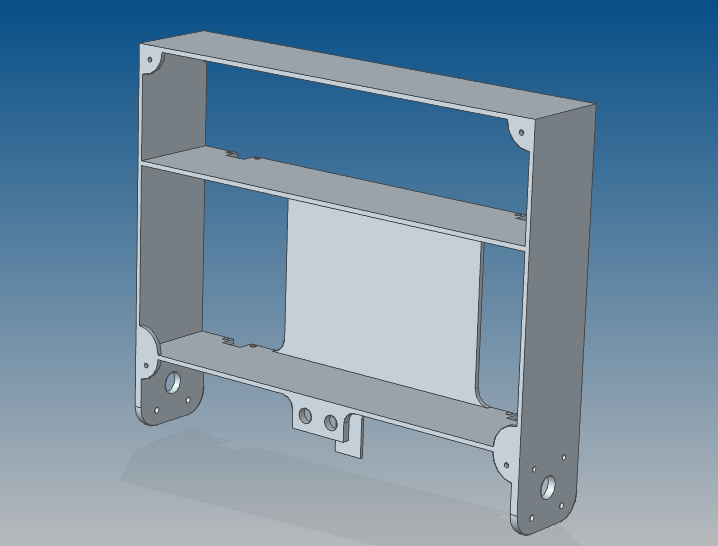
\includegraphics[width=0.5\textwidth]{images/gehaeuse-v1.png}
	% caption ist die Bildunterschrift, taucht auch im Abbildungsverzeichnis auf
	\caption{Gehäuse - V.1 \newline (Quelle: eigene Darstellung)}
	\label{gehaeuse-v1} % über das label kann man aus dem Text auf das Bild verweisen
\end{figure}
Es wurde gesagt, sehr einfachen Aufbau des Gehäuse im Form des Kasten herzustellen.
\subsection{Die Gehäusen - V.2}
\begin{figure}[!h]  % [h] bedeutet, dass das Bild genau an dieser Stelle im Text erscheint
	% mit width=... wird die Größe des Bildes in Prozent der Seitenbreite eingestellt
	\centering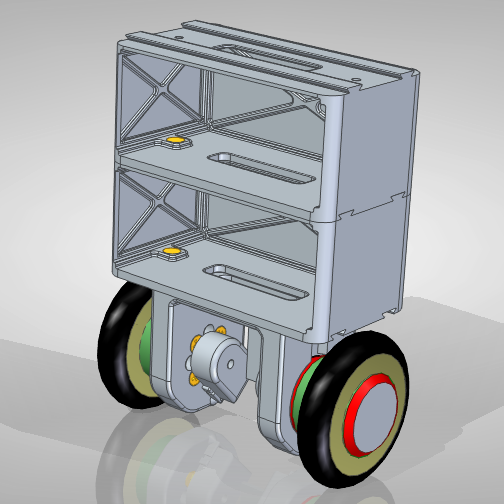
\includegraphics[width=0.5\textwidth]{images/gehaeuse-v2.png}
	% caption ist die Bildunterschrift, taucht auch im Abbildungsverzeichnis auf
	\caption{Gehäuse - V.2 \newline (Quelle: eigene Darstellung)}
	\label{gehaeuse-v2} % über das label kann man aus dem Text auf das Bild verweisen
\end{figure}
Im Bild \ref{gehaeuse-v2} ist eine modulare Darstellung des Roboters zu sehen. Das Motorhalter ist in diesem Fall als ein externer Modul dergestalt. Im ersten Modul von oben sollte man alle Steuerungsplatinen  einbauen. Das zweiten Modul von Oben sollte  das Akku beinhalten. Mit Hilfe vom Schwalbenschwanzverbindung und zwei Schrauben sollten die Module miteinander verbindet werden.

\subsection{Die Gehäusen - V.3}

Die Version V.2 (Bild \ref{gehaeuse-v2}) unterscheidet sich nicht viel von V.3. Es wurde die modulare Aufbau nicht geändert. Da hat man Schwalbenschwanzverbindung durch Steckverbindung ersetzt, die seitlich Zugeordnet sind. Es wurde auch Motorhalter modernisiert.

\begin{figure}[!h]  % [h] bedeutet, dass das Bild genau an dieser Stelle im Text erscheint
	% mit width=... wird die Größe des Bildes in Prozent der Seitenbreite eingestellt
	\centering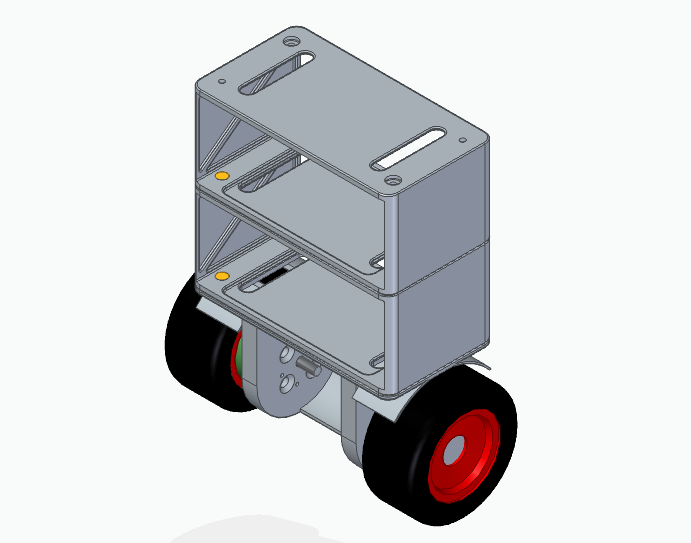
\includegraphics[width=0.5\textwidth]{images/gehaeuse-v3.png}
	% caption ist die Bildunterschrift, taucht auch im Abbildungsverzeichnis auf
	\caption{Gehäuse - V.2 \newline (Quelle: eigene Darstellung)}
	\label{gehaeuse-v3} % über das label kann man aus dem Text auf das Bild verweisen
\end{figure}

\subsection{Die Gehäusen - V.4}

Endgültige Gehäuse 

\begin{figure}[htb]
	\centering
	\begin{minipage}{0.45\linewidth}
		\centering
		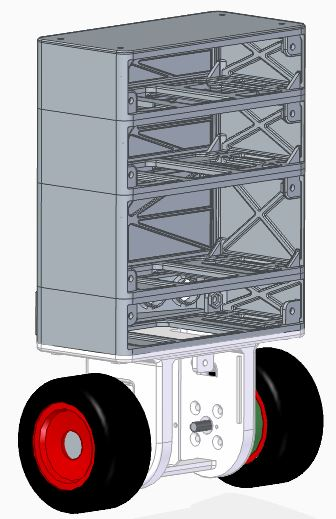
\includegraphics[scale=0.48]{images/4.1_vorne.jpg}
		\caption{Endgültige Gehäuse V4.1 \newline(Quelle: Eigene Darstellung)}
		\label{gehaeuse-v4}
	\end{minipage}
	%\hfill
	\begin{minipage}{0.45\linewidth}
		\centering
		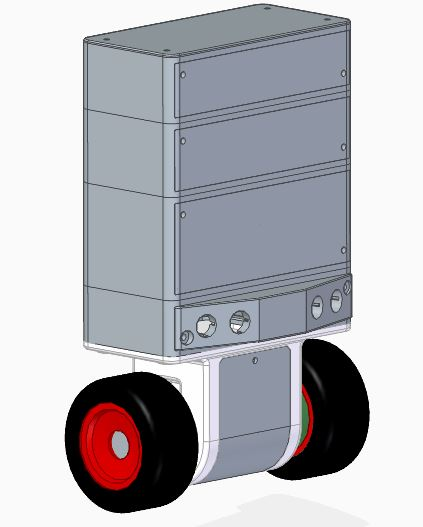
\includegraphics[scale=0.48]{images/4.1_hinten.jpg}
		\caption{ mit Deckels \newline (Quelle: Eigene Darstellung)}
	\end{minipage}
\end{figure}
\pagebreak
\subsection{Die Gehäusen - V.4.2.3}

Nach Zusammenbau des Roboters wurde folgende Korrektur noch durchgeführt:
 
\begin{itemize} 
	\item  mBed-Modul wurde 10 mm höher gemacht.
	\item  Anpassung an Kabelkanal Führung.
	\item  Beschriftung auf der Modulen.
	\item  Oberwand wurde komplett entfernt.
	\item  Versteifungen als Deckelsturzstelle.
	\item  Akku-Modul wurde 10 mm höher gemacht.
	\item  mBed und oDrive wurden stark nach einer Seite platziert.
\end{itemize}

\begin{figure}[htb]
	\centering
	\begin{minipage}{0.45\linewidth}
		\centering
		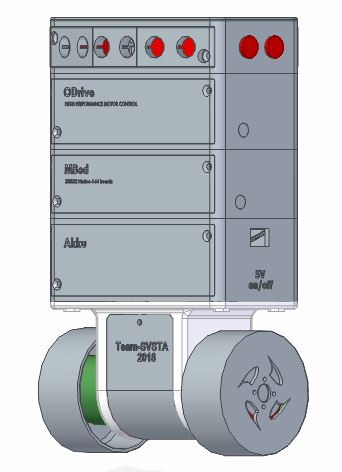
\includegraphics[scale=0.48]{images/V.4.3.jpg}
		\caption{Gehäuse V4.3 \newline(Quelle: Eigene Darstellung)}
		\label{gehaeuse-v4.3}
	\end{minipage}
	%\hfill
	\begin{minipage}{0.45\linewidth}
		\centering
		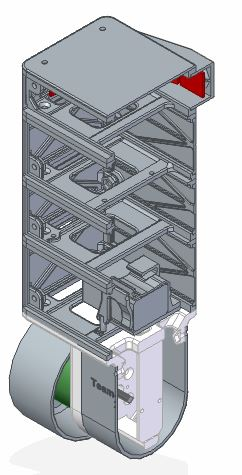
\includegraphics[scale=0.48]{images/V.4.3-1.jpg}
		\caption{ Schnitt \newline (Quelle: Eigene Darstellung)}
	\end{minipage}
\end{figure}
\pagebreak
\subsubsection{ Berechnung vom Motorhalter}
Alle Berechnungen wurden mit Hilfe von FEM - Programmierung gemacht und beweise die Festigkeit nur von dem Motorhalter. Es wurden an den Stellen vom Motoren und Räder das Moment laut der Berechnung \ref{FEM1} verwendet und als Lastkraft wurde 50N auf die Oberfläche eingeprägt.

Die Materialeigenschaften kann man aus der Abbildung \ref{FEM2} ablesen.

\begin{figure}[!h]  % [h] bedeutet, dass das Bild genau an dieser Stelle im Text erscheint
	\centering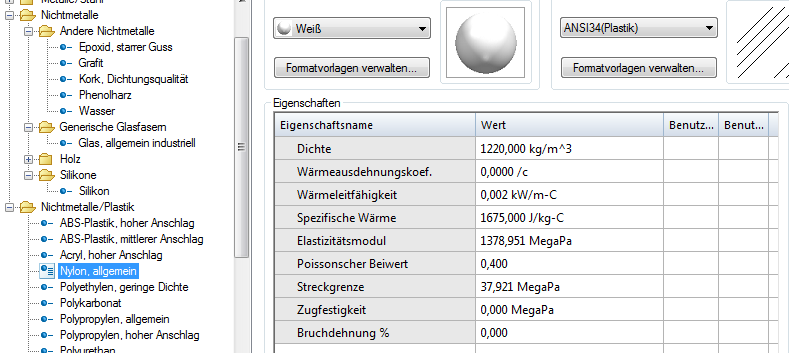
\includegraphics[width=0.7\textwidth]{images/FEM2.png}
	% caption ist die Bildunterschrift, taucht auch im Abbildungsverzeichnis auf
	\caption{Kunststoffeigenschaften - Nylon (PA) \newline (Quelle: eigene Darstellung)}
	\label{FEM2} % über das label kann man aus dem Text auf das Bild verweisen
\end{figure}
\begin{figure}[!h]  % [h] bedeutet, dass das Bild genau an dieser Stelle im Text erscheint
	% mit width=... wird die Größe des Bildes in Prozent der Seitenbreite eingestellt
	\centering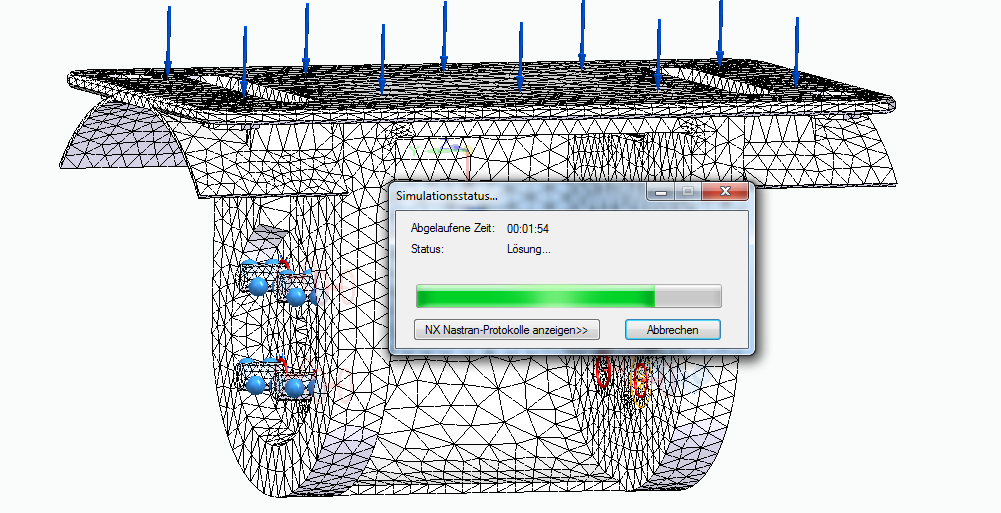
\includegraphics[width=0.9\textwidth]{images/FEM.png}
	% caption ist die Bildunterschrift, taucht auch im Abbildungsverzeichnis auf
	\caption{FEM-Berechnung \newline (Quelle: eigene Darstellung)}
	\label{FEM1} % über das label kann man aus dem Text auf das Bild verweisen
\end{figure}
\begin{figure}[!h]  % [h] bedeutet, dass das Bild genau an dieser Stelle im Text erscheint
	\centering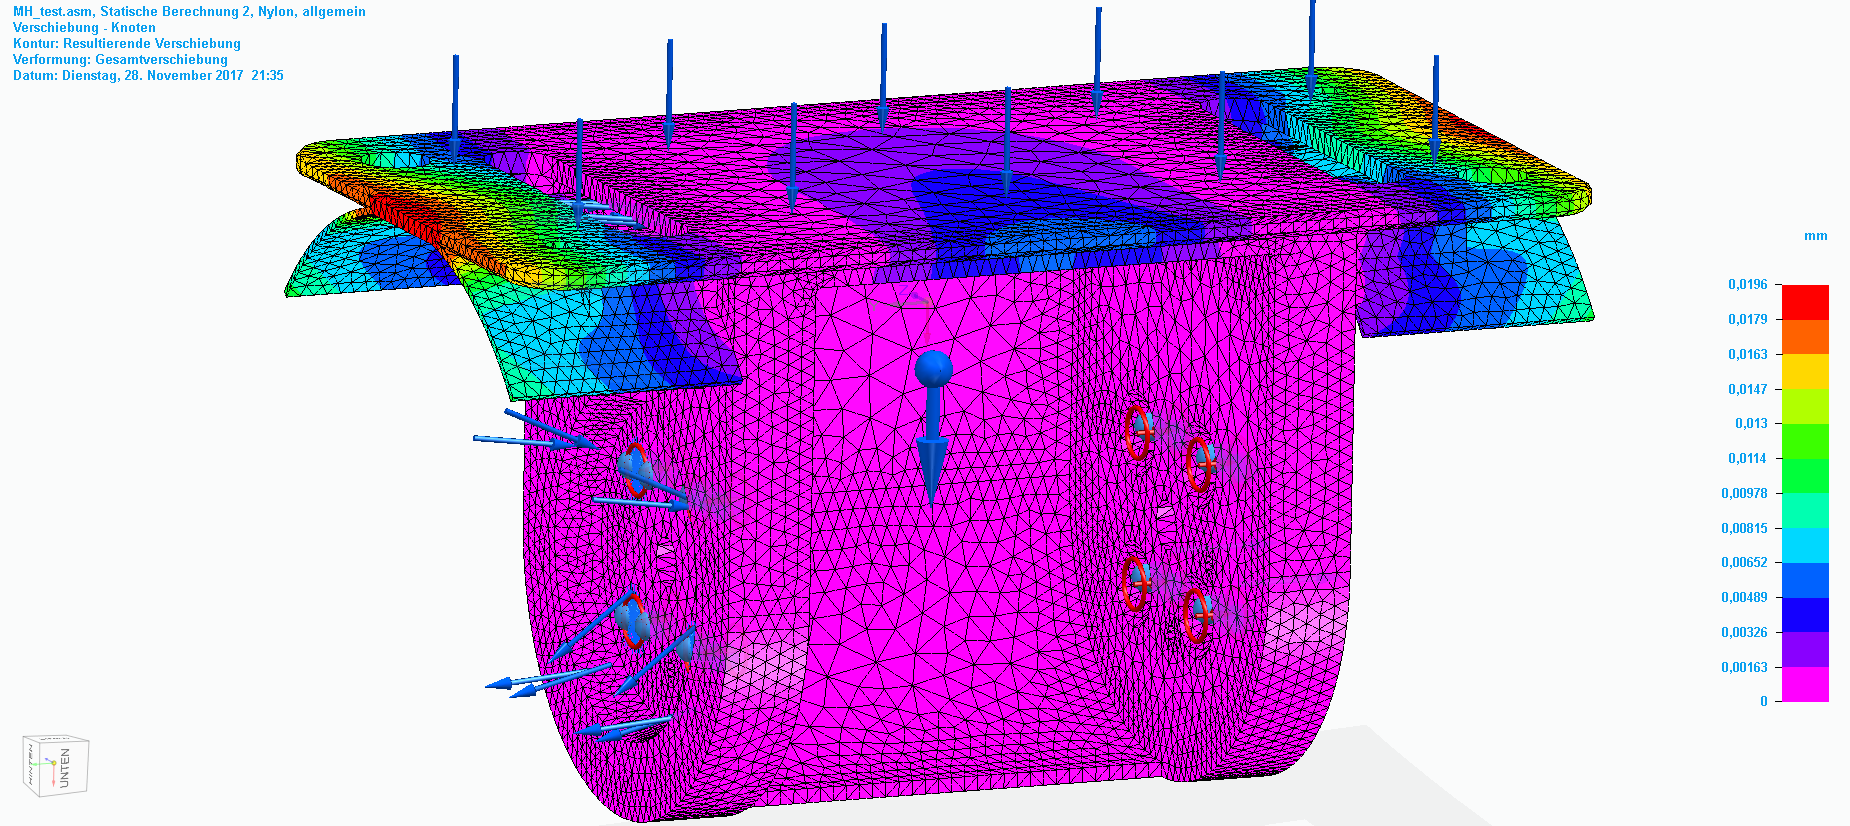
\includegraphics[width=0.9\textwidth]{images/FEM3.png}
	% caption ist die Bildunterschrift, taucht auch im Abbildungsverzeichnis auf
	\caption{FEM - Verschiebungen \newline (Quelle: eigene Darstellung)}
	\label{FEM3} % über das label kann man aus dem Text auf das Bild verweisen
\end{figure}
\pagebreak
Sicherheitsfaktor ....

\begin{figure}[!h]  % [h] bedeutet, dass das Bild genau an dieser Stelle im Text erscheint
	\centering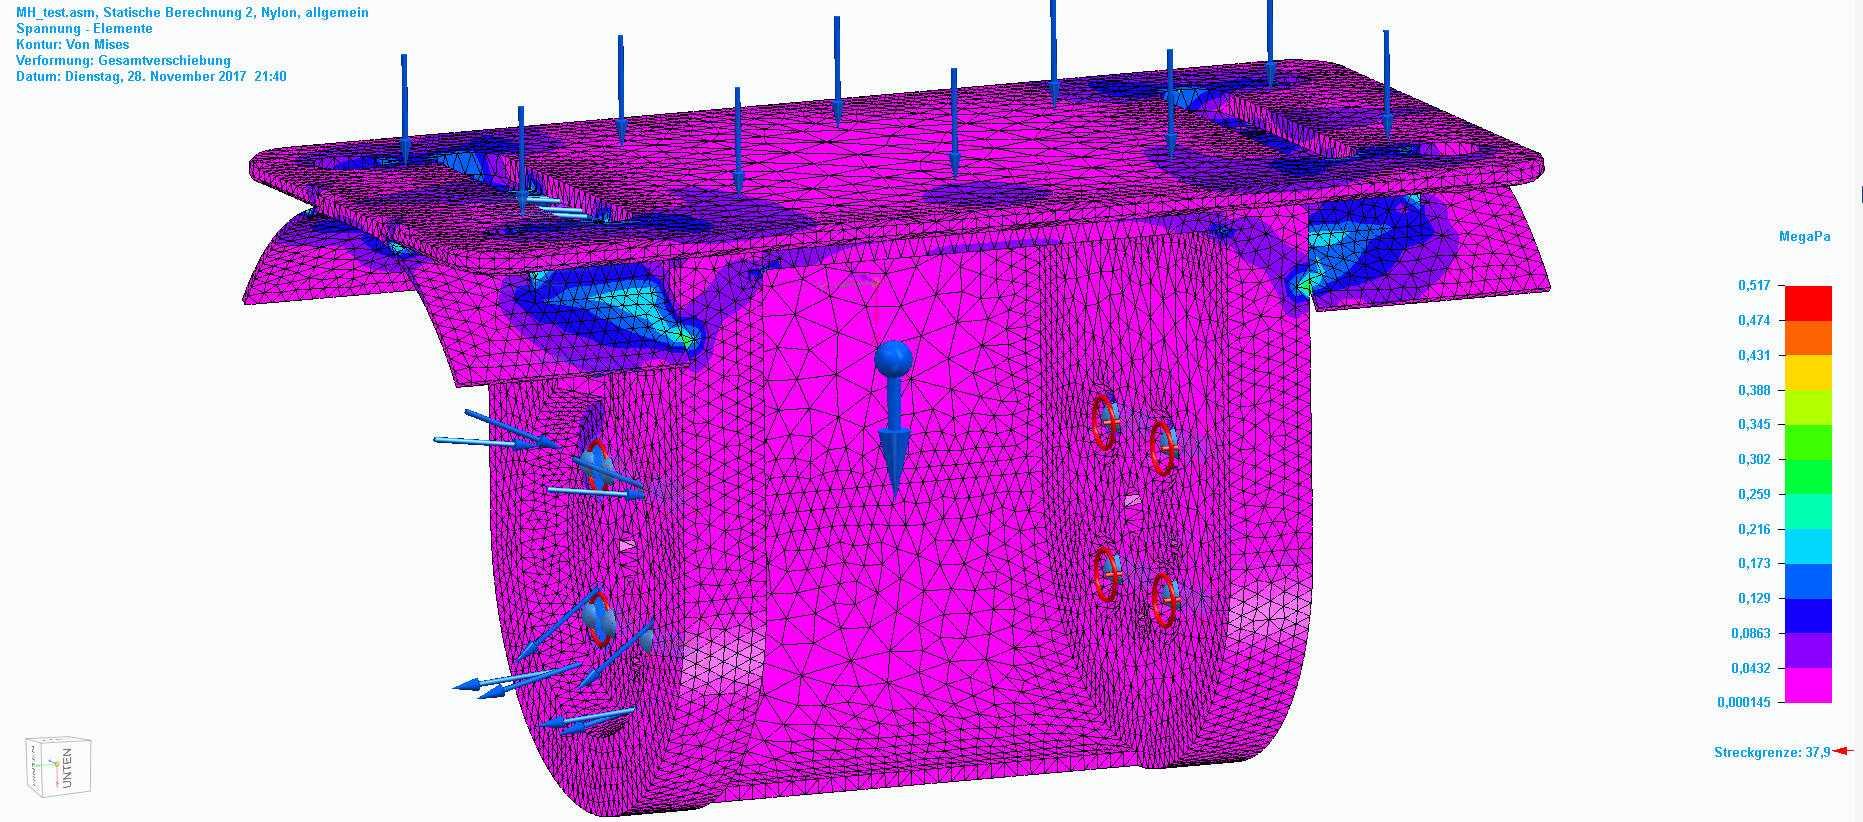
\includegraphics[width=0.9\textwidth]{images/FEM4.png}
	% caption ist die Bildunterschrift, taucht auch im Abbildungsverzeichnis auf
	\caption{FEM - Spannungen \newline (Quelle: eigene Darstellung)}
	\label{FEM4} % über das label kann man aus dem Text auf das Bild verweisen
\end{figure}
\pagebreak

